\documentclass[12pt,a4paper]{article}
\usepackage[utf8]{inputenc}
\usepackage[T1]{fontenc}
\usepackage{amsmath}
\usepackage{amsfonts}
\usepackage{amssymb}
\usepackage{graphicx}
\usepackage{hyperref}
\usepackage{listings}
\usepackage{xcolor}
\usepackage{geometry}
\usepackage{dirtree}
\usepackage{fancyhdr}
\usepackage{lastpage}
\geometry{margin=1in}
\lstset{
  backgroundcolor=\color{white},
  basicstyle=\footnotesize\ttfamily,
  breakatwhitespace=false,
  breaklines=true,
  captionpos=b,
  commentstyle=\color{green},
  extendedchars=true,
  frame=single,
  keepspaces=true,
  keywordstyle=\color{blue},
  language=Bash,
  numbers=left,
  numbersep=5pt,
  numberstyle=\tiny\color{gray},
  rulecolor=\color{black},
  showspaces=false,
  showstringspaces=false,
  showtabs=false,
  stepnumber=1,
  stringstyle=\color{purple},
  tabsize=2,
  title=\lstname
}
\pagestyle{fancy}
\fancyhf{}
\rhead{GeoTools Package Manual}
\lhead{Caio Ciardelli}
\rfoot{Page \thepage\ of \pageref{LastPage}}
\title{GeoTools Package Manual}
\author{Caio Ciardelli \\ Northwestern University \\ Under the supervision of Prof. Suzan van der Lee}
\date{January 2026}
\begin{document}
\maketitle
\tableofcontents
\newpage
\section{Introduction}
The GeoTools Package is a geosciences software package developed for computing seismic ray paths, travel times, and synthetic gravity disturbances in 3D Earth models, including surface topography. It is written in C, Python, and Bash, and is designed for high-performance computations using parallel processing (via OpenMPI). The package is currently under development and focuses on forward modeling capabilities. The package now includes the capability to incorporate Moho topography into the mesh, affecting both gravity calculations and travel time computations. For travel times, Moho topography is accounted for by locally deforming the ray path, which serves as an approximation until full 3D ray tracing is implemented. Future versions will include inversion features for 3D velocity and density distributions, 3D ray tracing, and Earth's ellipticity.
This manual provides a comprehensive guide to installing, compiling, running, and understanding the package. It includes details on the directory structure, dependencies, key scripts and programs, input/output files, and usage examples.
The program is licensed under the GNU General Public License (GPL) version 3 or later. See the LICENSE file for details.

\section{Dependencies}
The GeoTools Package requires the following software and libraries:

\begin{itemize}
    \item \textbf{Bash}: For running shell scripts (e.g., run\_test\_workflow.bash, plot\_mesh.bash, plot\_gravity.bash).
    \item \textbf{GCC}: C compiler for building the C binaries (mesher, gravity, ttimes).
    \item \textbf{Python 3.7 or later}: For Python scripts (compute\_rays.py, resample\_1d\_model.py, pvsm\_generator.py).
    \item \textbf{Python libraries}:
        \begin{itemize}
            \item NumPy>1.26.4: Data processing and arrays (used in compute\_rays.py, resample\_1d\_model.py).
            \item Matplotlib>3.7.2: Plotting (used in resample\_1d\_model.py and optionally in compute\_rays.py).
            \item PvPython>3.12.7: Python with Paraview bindings (required for pvsm\_generator.py).
            \item OpenMPI>5.0: OpenMPI for parallel execution (required for gravity field computation).
            \item SeisTracer: Seismic ray tracing library (required for compute\_rays.py).
            \item argparse: Command-line parsing (standard library).
            \item heapq, math: Standard libraries for algorithms and calculations.
            \item os, shutil: Standard libraries for file handling.
        \end{itemize}
    \item \textbf{GMT (Generic Mapping Tools)}: For generating plots (used in plot\_mesh.bash and plot\_gravity.bash).
    \item \textbf{ParaView}: Installation with Python support for 3D visualization (pvsm\_generator.py generates .pvsm state files for interactive rendering).
    \item \textbf{OpenMPI}: For parallel execution in gravity.c (uses MPI for distributed computing across multiple cores).
    \item \textbf{bc}: Basic calculator for arithmetic operations in plot\_gravity.bash.
\end{itemize}

Ensure all dependencies are installed on your system. For Python libraries, use pip:

\begin{lstlisting}[language=Bash]
pip install numpy matplotlib paraview
\end{lstlisting}

Note: SeisTracer requires additional installation steps; refer to its documentation. The package assumes access to ETOPO topography data in extra/earth\_relief\_15m.topo for surface topography incorporation and CRUST1.0 Moho data in extra/crust1\_moho.dat for Moho topography incorporation.

\section{Directory Structure}
The package is organized as follows:

\dirtree{%
.1 .
.2 docs.
.3 Manual.pdf.
.3 Manual.tex.
.2 extra.
.3 CET-D01A.cpt.
.3 crust1\_moho.dat.
.3 earth\_relief\_15m.topo.
.2 input.
.3 receivers.dat.
.3 sources.dat.
.2 LICENSE.
.2 Makefile.
.2 mesh.
.3 facets.bin.
.3 Mesh\_VpVsRho.vtk.
.3 r.bin.
.3 rho.bin.
.3 vertices.bin.
.3 vp.bin.
.3 vs.bin.
.2 models.
.3 ak135f.model.
.3 iasp91.model.
.3 prem.model.
.3 rem1d.model.
.3 stw105.model.
.2 README.md.
.2 run\_test\_workflow.bash.
.2 setup.
.3 constants.h.
.2 src.
.3 gravity.c.
.3 headers.
.4 coordinates.h.
.4 exmath.h.
.4 io.h.
.4 progress.h.
.4 structs.h.
.4 tesselation.h.
.3 mesher.c.
.3 shared.
.4 coordinates.c.
.4 exmath.c.
.4 io.c.
.4 progress.c.
.4 tesselation.c.
.3 ttimes.c.
.2 utils.
.3 compute\_rays.py.
.3 plot\_gravity.bash.
.3 plot\_mesh.bash.
.3 pvsm\_generator.py.
.3 resample\_1d\_model.py.
}

Key directories:

\begin{itemize}
    \item \textbf{extra}: Contains topography data (ETOPO: earth\_relief\_15m.topo), Moho data (CRUST1.0: crust1\_moho.dat), and color palettes (CET-D01A.cpt) for GMT plotting.
    \item \textbf{input}: Input files for receivers (receivers.dat: station ID, lat, lon, elevation) and sources (sources.dat: event ID, lat, lon, depth) used in ray tracing.
    \item \textbf{mesh}: Output directory for mesh-related binary files (e.g., facets.bin, vertices.bin, r.bin, rho.bin, vp.bin, vs.bin) and VTK files (Mesh\_VpVsRho.vtk).
    \item \textbf{models}: Predefined 1D Earth models (e.g., iasp91.model, prem.model) in text format for resampling and meshing.
    \item \textbf{setup}: Configuration header (constants.h) for C programs, controlling flags like INCORPORATE\_SURFACE\_TOPOGRAPHY (default: true) and DEBUG\_MESH (default: true).
    \item \textbf{src}: C source code, including main programs (mesher.c, gravity.c, ttimes.c), headers, and shared utilities for math, I/O, and tesselation.
    \item \textbf{utils}: Utility scripts in Python and Bash for model resampling, ray computation, plotting, and ParaView state generation.
\end{itemize}

\section{Compilation}
The package uses a Makefile in the root directory for compilation. To build the C binaries (mesher, gravity, ttimes):

\begin{lstlisting}[language=Bash]
make all
\end{lstlisting}

This compiles the source files in src/ (using headers from src/headers and shared code from src/shared) and places the executables in a new bin/ directory. The compilation requires GCC and OpenMPI for parallel support in gravity.
To clean previous build artifacts:

\begin{lstlisting}[language=Bash]
make clean
\end{lstlisting}
Note: Ensure GCC and OpenMPI are in your PATH. The Makefile assumes standard includes; modify it if needed for custom library paths. After compilation, grant execution permissions to utility scripts if necessary (e.g., chmod +x utils/*.bash).

\section{Running the Program}
The main entry point is the test workflow script: run\_test\_workflow.bash. It automates the entire forward modeling process: model resampling, ray path computation, mesh generation, travel time calculation, gravity computation, and visualizations. The script uses a fixed refinement level (7), model (IASP91), and parameters (e.g., NCORES=6, DELTA=5.0, HEIGHT=255 km), but these can be customized by editing the script.

Usage:

\begin{lstlisting}[language=Bash]
./run_test_workflow.bash
\end{lstlisting}

Steps performed by the script:

\begin{itemize}
    \item Cleans previous outputs (removes phases directories, .txt, .dat, .png, .vtk, .pvsm, gmt.history).
    \item Resamples the 1D IASP91 model to input/input.model using resample\_1d\_model.py.
    \item Computes ray paths for sample source/receiver pairs using compute\_rays.py, outputting to phases\_EQ001\_STA01/.
    \item Generates the mesh with refinement 7 using mesher.
    \item Plots the mesh with plot\_mesh.bash, creating PNGs like mesh320.png and nodes\_spiral.png.
    \item Generates a ParaView state file (e.g., Mesh\_VpVsRho.pvsm) with pvsm\_generator.py for mesh and selected phases (PKIIKP, etc.).
    \item Computes travel times for phases in phases\_EQ001\_STA01/ using ttimes, outputting to ttimes.txt.
    \item Computes synthetic gravity in parallel (mpiexec -n 6) using gravity with DELTA=5.0 and HEIGHT=255, outputting G\_*.dat files. Note: Requires ~16 GB RAM; reduce NCORES, layers, or refinement if memory is limited.
    \item Plots gravity with plot\_gravity.bash on G\_normal.dat, creating G\_normal.png.
\end{itemize}

For help:

\begin{lstlisting}[language=Bash]
./run_test_workflow.bash --help
\end{lstlisting}

Individual components can be run manually (see Section 6). Outputs are placed in the current directory or subdirectories like mesh/ and phases\_EQ001\_STA01/.

\section{Key Components and Usage}
\subsection{resample\_1d\_model.py (utils/resample\_1d\_model.py)}
This Python script resamples a 1D Earth model in two stages: linear collapse (removes points in constant-gradient intervals) and importance-based pruning (removes least important points until target ratio). It preserves header lines and outputs stats, errors, and an optional comparison plot.
Usage:

\begin{lstlisting}[language=Bash]
python utils/resample_1d_model.py -i INPUT -o OUTPUT [options]
\end{lstlisting}

Key options (from argparse):

\begin{itemize}
    \item -i, --input: Input model file (required, e.g., models/iasp91.model).
    \item -o, --output: Output resampled model file (required).
    \item --depth-col: Depth column index (default: 0).
    \item --check-cols: Columns to resample (default: all except depth).
    \item --rtol: Relative slope tolerance for linear collapse (default: 1e-6).
    \item --atol: Absolute slope tolerance (default: 1e-8).
    \item --target-keep-ratio: Fraction of points to keep (default: 0.50).
    \item --normalize: Normalize errors by column range (default: True).
    \item --error-agg: Error aggregation method (default: max).
    \item --preserve-zero: Preserve points where any checked column is zero (default: True).
    \item --enable-linear: Enable linear collapse stage (default: True).
    \item --save-fig: Save comparison plot as OUTPUT.png.
    \item --max-cols: Max columns to plot (default: 4).
    \item --header-lines: Header lines to preserve (default: 4).
    \item --fortran-d: Handle Fortran D notation (default: True).
\end{itemize}

Input: Text file with header (4 lines) and data columns (e.g., depth, Vp, Vs, rho).
Output: Resampled model file, console stats (reduction \%, max errors), optional PNG plot.
Example (from workflow): python utils/resample\_1d\_model.py -i models/iasp91.model -o input/input.model

\begin{figure}[!h]
  \centering
  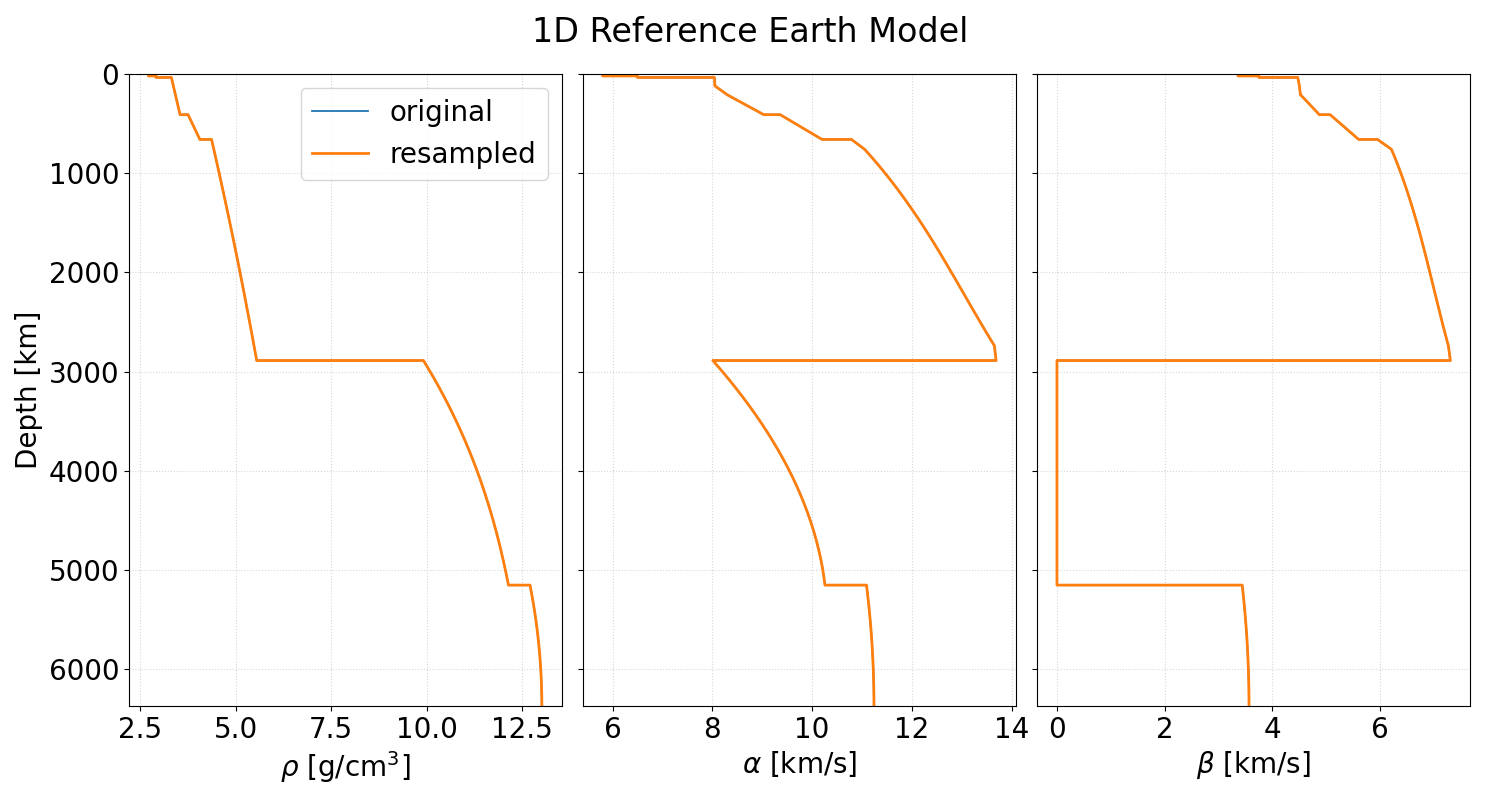
\includegraphics[width=0.8\textwidth]{figs/1d_model_resampling.png}
  \caption{Comparison between the original and resampled 1D reference Earth model.}
\end{figure}

\subsection{compute\_rays.py (utils/compute\_rays.py)}
This Python script computes seismic ray paths for source-receiver pairs using SeisTracer. It generates directories with VTK/text files for rays, phase lists, and optional PNG plots. Supports multiple phases and saves receiver elevation.
Usage:

\begin{lstlisting}[language=Bash]
python utils/compute_rays.py -r RECEIVERS -s SOURCES [options]
\end{lstlisting}

Key options:

\begin{itemize}
    \item -r: Receivers file (required, e.g., input/receivers.dat: ID lat lon elev).
    \item -s: Sources file (required, e.g., input/sources.dat: ID lat lon depth).
    \item --no-png: Disable PNG ray path plots.
    \item --no-vtk: Disable VTK ray path files.
\end{itemize}

Input: receivers.dat and sources.dat (text files with locations).
Output: Directory per pair (e.g., phases\_EQ001\_STA01/) with:

\begin{itemize}
    \item PHASE.vtk / PHASE.txt: Ray coordinates and branches.
    \item sr.vtk: Source/receiver points.
    \item phases\_list.txt: List of computed phases.
    \item receiver\_elevation.txt: Receiver elevation in meters.
    \item Optional PHASE.png: Ray path plots.
\end{itemize}

Example (from workflow): python utils/compute\_rays.py -r input/receivers.dat -s input/sources.dat
Notes: Uses Vincenty's formula for great-circle distances; maps branch types (P=0, S=1).

\begin{figure}[!h]
  \centering
  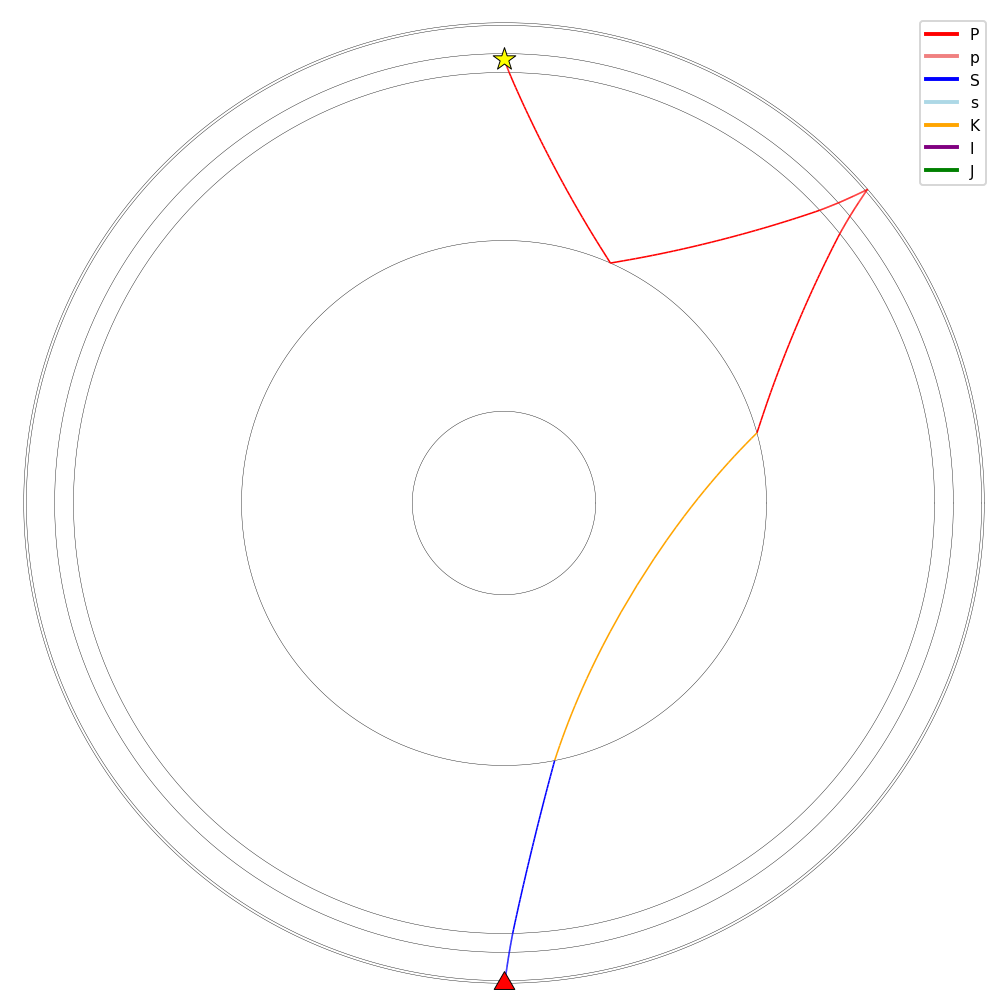
\includegraphics[width=0.5\textwidth]{figs/PcPPKSSm+S.png}
  \caption{Example of a single seismic ray path computed for a complex phase.}
\end{figure}

\begin{figure}[!h]
  \centering
  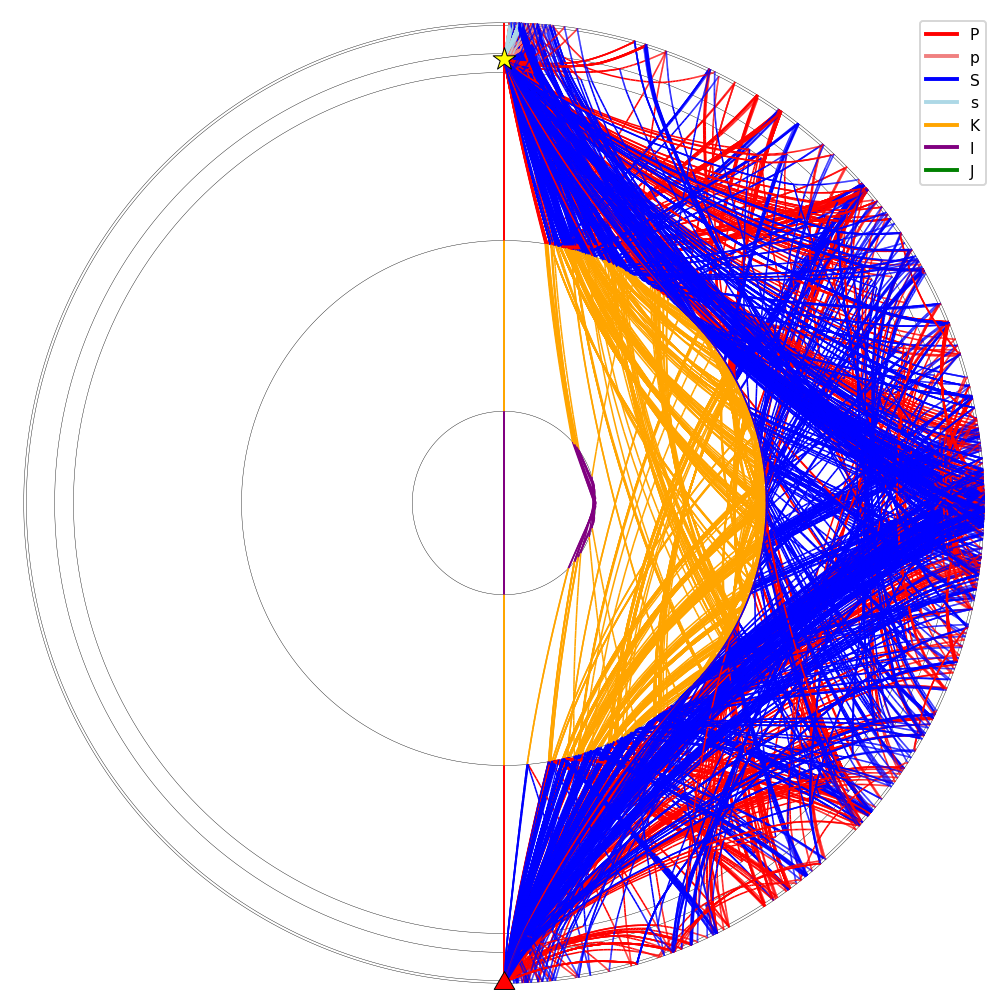
\includegraphics[width=0.5\textwidth]{figs/ray_paths_EQ001_STA01.png}
  \caption{Multiple seismic ray paths for various phases between a source and receiver pair.}
\end{figure}

\subsection{mesher.c (bin/mesher)}
This C program creates a spherical mesh based on a 1D velocity model, optionally incorporating ETOPO topography (with Gaussian anti-aliasing filter), CRUST1.0 Moho topography (similarly filtered), and 3D perturbations. Starts from an icosahedron and refines it. The Moho topography is incorporated by adjusting the radii at the Moho discontinuity level, using a similar anti-aliasing filter as for surface topography. By default, it uses the Moho depths from the CRUST1.0 model in extra/crust1\_moho.dat, but users can specify a different file by changing the variable 
\lstinline{MOHO_FILE_NAME} in constants.h.

Usage:

\begin{lstlisting}[language=Bash]
./bin/mesher REFINEMENT MODEL
\end{lstlisting}

\begin{itemize}
    \item REFINEMENT: Number of refinement iterations (e.g., 7; increases vertices/facets exponentially).
    \item MODEL: Path to 1D model file (e.g., input/input.model).
\end{itemize}

Output (in mesh/ and current dir):

\begin{itemize}
    \item Binary: facets.bin (facet data), vertices.bin (vertex data), r.bin/rho.bin/vp.bin/vs.bin (model values per vertex/shell).
    \item Text: nodes.txt (lon/lat of vertices), spiral.txt (spiral-ordered vertices), mesh\_edges\_\%d.txt, mesh\_triangles\_\%d.txt, mesh\_center\_triangle\_\%d.txt (for DEBUG\_MESH=true).
    \item VTK: Mesh\_VpVsRho.vtk (3D mesh with Vp, Vs, Rho scalars).
\end{itemize}

Configurable in constants.h:

\begin{itemize}
    \item INCORPORATE\_SURFACE\_TOPOGRAPHY: true (uses extra/earth\_relief\_15m.topo).
    \item INCORPORATE\_MOHO\_TOPOGRAPHY: true (uses extra/crust1\_moho.dat).
    \item INCORPORATE\_3D\_MODEL: false (placeholder for 3D perturbations).
    \item DEBUG\_MESH: true (outputs text files for plotting).
\end{itemize}

Example (from workflow): ./bin/mesher 7 input/input.model
Notes: Prints mesh stats (facets, vertices, edge lengths). Requires ~ number of shells from model.

\begin{figure}[!h]
  \centering
  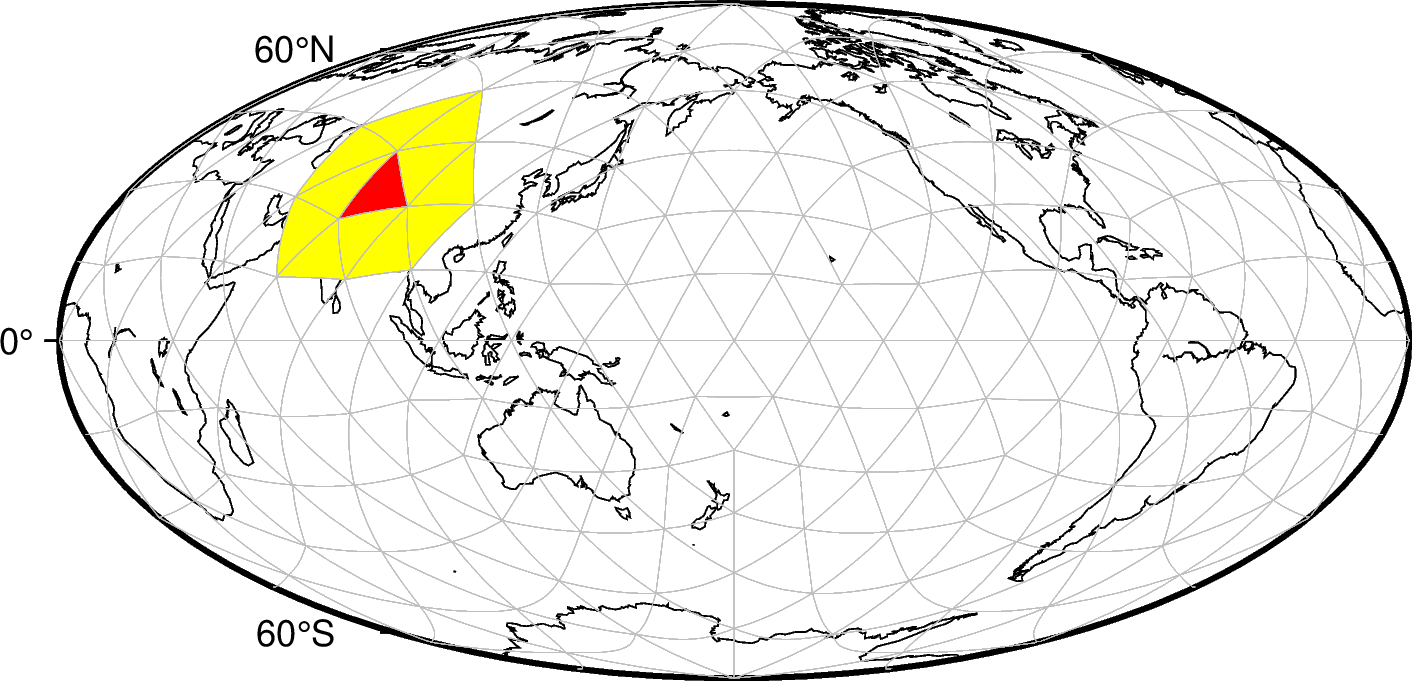
\includegraphics[width=0.8\textwidth]{figs/mesh320.png}
  \caption{Global map showing a highlighted triangle in the spherical mesh.}
\end{figure}

\begin{figure}[!h]
  \centering
  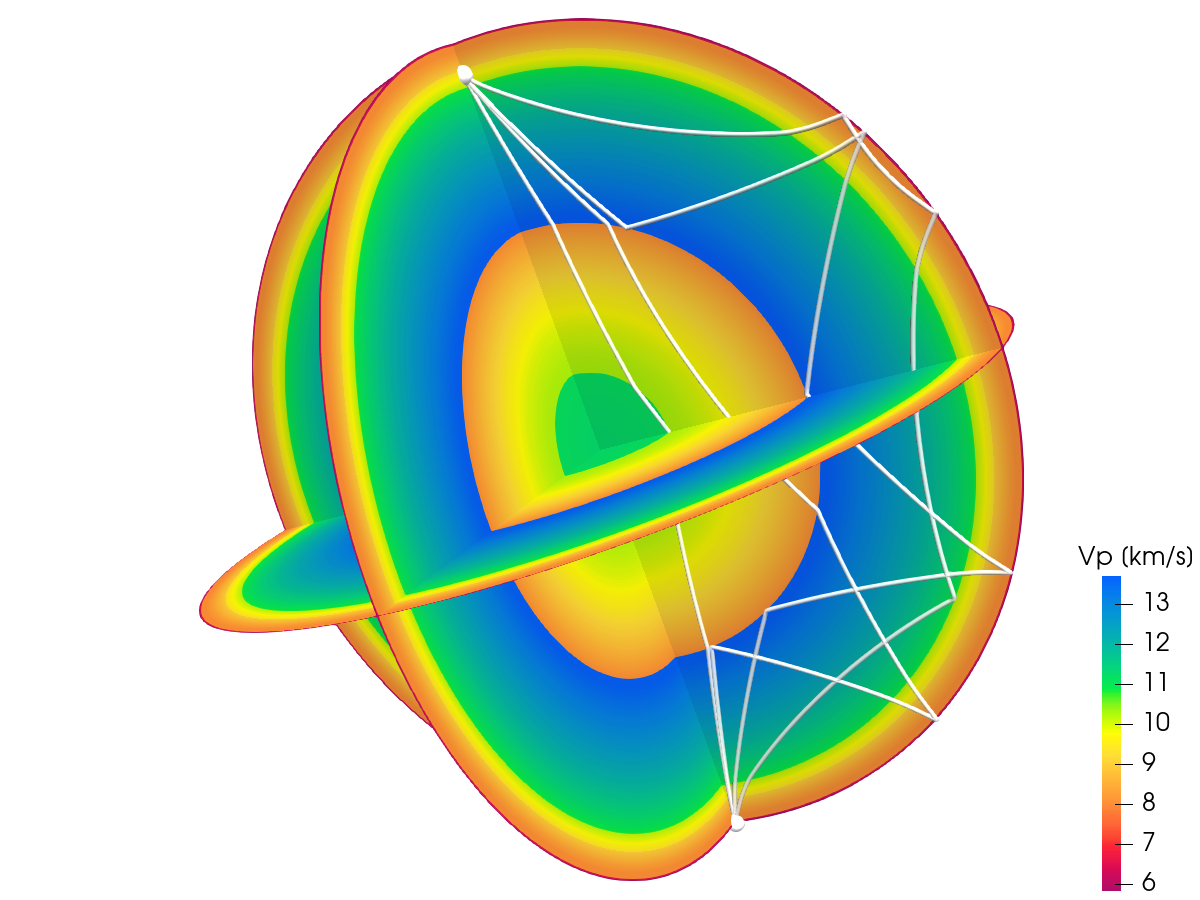
\includegraphics[width=1.0\textwidth]{figs/Mesh_Visualization.png}
  \caption{3D visualization of the mesh colored by P-wave velocity (Vp).}
\end{figure}

\subsection{ttimes.c (bin/ttimes)}
This C program computes seismic travel times for phases using the mesh and model, accounting for topography via receiver elevation. When Moho topography is incorporated (via INCORPORATE\_MOHO\_TOPOGRAPHY in constants.h), it is accounted for by locally deforming the ray path near the Moho discontinuity. This deformation adjusts the ray to follow the varying Moho depth, providing an approximation to the true 3D path perturbation caused by the Moho topography. This is an interim solution; the ideal approach of full 3D ray tracing will replace this approximation in future versions.

Usage:

\begin{lstlisting}[language=Bash]
./bin/ttimes INPUT_DIR > ttimes.txt
\end{lstlisting}

\begin{itemize}
    \item INPUT\_DIR: Directory with phases\_list.txt (phase names) and PHASE.txt (ray coordinates/branches), receiver\_elevation.txt.
\end{itemize}

Output: To stdout: Phase names and travel times (seconds).
Example (from workflow): ./bin/ttimes phases\_EQ001\_STA01/ > ttimes.txt
Notes: Reads mesh/model binaries; resamples rays with DELTA=0.1 km; uses barycentric coordinates for element location.

\subsection{gravity.c (bin/gravity)}
This C program computes Earth's gravitational field in parallel using MPI, accounting for topography and height. When Moho topography is incorporated into the mesh (via INCORPORATE\_MOHO\_TOPOGRAPHY in constants.h), it affects the gravity calculations by altering the density distribution at the Moho level in the 3D model.
Usage:

\begin{lstlisting}[language=Bash]
mpiexec -n NCORES ./bin/gravity DH HEIGHT
\end{lstlisting}

\begin{itemize}
    \item DH: Grid spacing in degrees (e.g., 5.0).
    \item HEIGHT: Observation height in km (e.g., 255).
\end{itemize}

Output: G\_x.dat, G\_y.dat, G\_z.dat (gravity components), G\_normal.dat (normal component, in g [m/s²]).
Notes: Reads mesh/model binaries; decomposes elements into tetrahedra; computes mass (prints Earth's mass). Parallel over facets.
Example (from workflow): mpiexec -n 6 ./bin/gravity 5.0 255

\subsection{plot\_mesh.bash (utils/plot\_mesh.bash)}
This Bash script generates GMT plots of mesh triangles, centers, and edges from text files.

Usage:

\begin{lstlisting}[language=Bash]
./utils/plot_mesh.bash
\end{lstlisting}

Input: Auto-detects mesh\_*.txt files in current directory.
Output: PNGs like mesh\%d.png (triangles in yellow, centers in red, edges in gray if <=20480), nodes\_spiral.png (if max=320: edges, spiral in magenta, nodes in green).
Example (from workflow): ./utils/plot\_mesh.bash

\subsection{plot\_gravity.bash (utils/plot\_gravity.bash)}
This Bash script generates a GMT plot of gravity data (e.g., normal component).

Usage:

\begin{lstlisting}[language=Bash]
./utils/plot_gravity.bash FILENAME
\end{lstlisting}

\begin{itemize}
    \item FILENAME: Base name without .dat (e.g., G\_normal).
\end{itemize}

Input: FILENAME.dat (lon lat gravity).
Output: FILENAME.png (global map with colorbar in mGal, using extra/CET-D01A.cpt).
Example (from workflow): ./utils/plot\_gravity.bash G\_normal
Notes: Grids data with xyz2grd/surface; rescales to mGal; avoids poles.

\begin{figure}[!h]
  \centering
  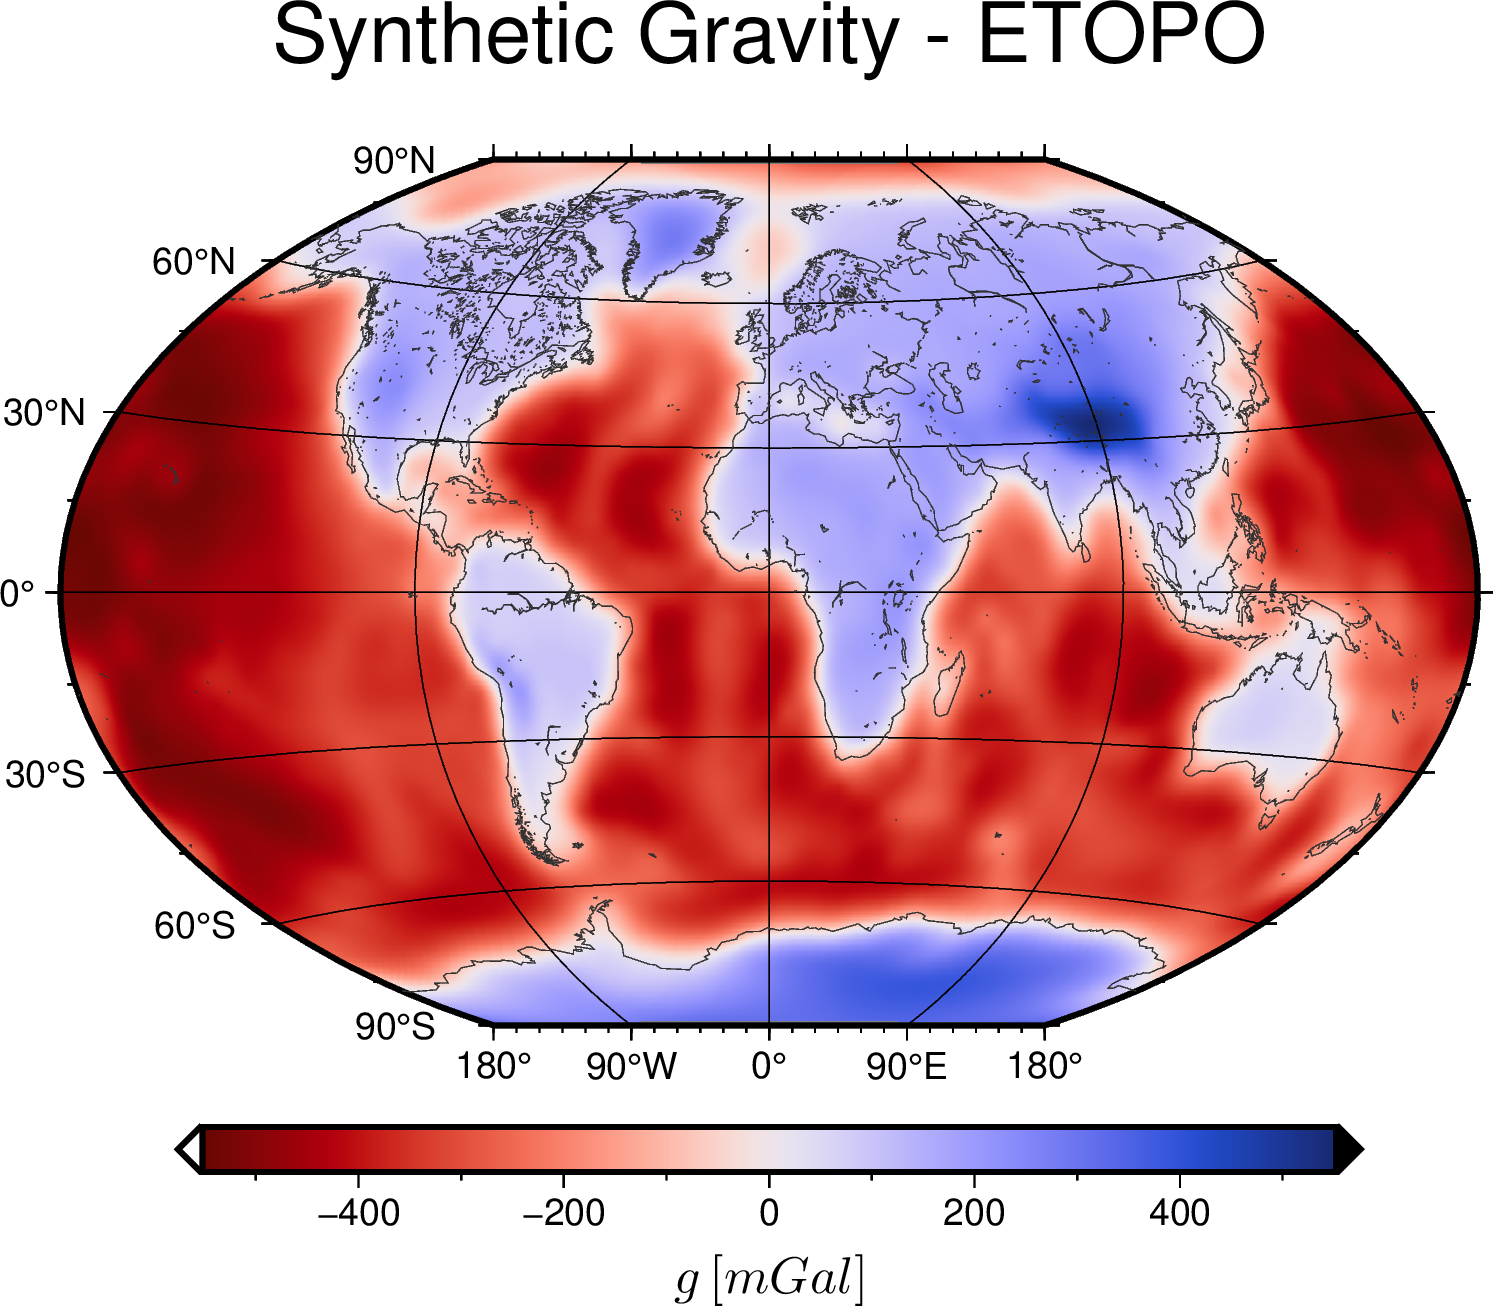
\includegraphics[width=0.8\textwidth]{figs/G_normal.png}
  \caption{Synthetic gravity map incorporating ETOPO topography (Moho topography was set to `false' in this example).}
\end{figure}

\subsection{pvsm\_generator.py (utils/pvsm\_generator.py)}
This Python script generates ParaView .pvsm state files for VTK mesh/ray visualization.
Usage:

\begin{lstlisting}[language=Bash]
pvpython utils/pvsm_generator.py MESH_VTK [options]
\end{lstlisting}

Key options:

\begin{itemize}
    \item --color-by: Scalar to color by (e.g., Vp).
    \item --phases-dir: Directory with ray VTKs.
    \item --phases: Space-separated phases (e.g., P S).
    \item --reverse-colormap: Reverse color map.
    \item --camera-view: View angles (e.g., 210,10,0,0,20).
    \item --light-intensity/azimuth/elevation: Light settings.
    \item --label: Colorbar label (e.g., 'Vp [km/s]').
\end{itemize}

Output: MESH\_VTK.pvsm (ParaView state file).
Example (from workflow): pvpython utils/pvsm\_generator.py mesh/Mesh\_VpVsRho.vtk --color-by Vp --phases-dir phases\_EQ001\_STA01 --phases PKIIKP PKPPm+PPcS ScSScSm-ScS SPS660-S --reverse-colormap --camera-view 210,10,0,0,20 --label 'Vp [km/s]' --light-intensity 0.5 --light-azimuth 140 --light-elevation 35
Notes: Requires pvpython or ParaView Python env; adds rays as tubes, sources/receivers as spheres.

\section{Examples}
Run the full test workflow:

\begin{lstlisting}[language=Bash]
./run_test_workflow.bash
\end{lstlisting}

This uses sample input/sources.dat (one event) and input/receivers.dat (one station), processes IASP91, and generates all outputs.
Customize rays: Edit input/sources.dat and receivers.dat for multiple events/stations.
View in ParaView: Load Mesh\_VpVsRho.pvsm for interactive 3D mesh/rays.
Run mesher standalone: ./bin/mesher 8 models/prem.model
Plot custom gravity: ./utils/plot\_gravity.bash my\_gravity

\section{Future Features}
\begin{itemize}
    \item 3D ray tracing in ttimes.
    \item Earth's ellipticity corrections.
    \item Inversion capabilities for 3D velocity/density and Moho topography.
\end{itemize}

For contributions or issues, contact the author.
\end{document}
